\documentclass[a4paper, 12pt, titlepage]{scrartcl}
\usepackage{authblk}

%============================================ Define Titlepage =====================================================%
     
\author[*]{\large Andreas Hill}
\author[ ]{\large Henning Buddenbaum}
\author[ ]{\large Daniel Mandallaz}
\affil[*]{\small Corresponding author: \underline{andreas.hill@usys.ethz.ch}}
\renewcommand\Authands{, } 

\date{\vspace{-0.8ex}}
\title{\LARGE Combining canopy height and tree species information for large scale timber volume estimations under strong heterogeneity of auxiliary data and variable sample plot sizes \vspace{-1ex}}
\subject{\vspace{-1.5cm} European Journal of Forest Research \\ \vspace{0.2cm} Supplementary Material \vspace{0.2cm} \vspace{-0.5cm}}


%============================================ Load Packages ========================================================%
\usepackage{geometry}
 \geometry{
 a4paper,
 left=20mm,
 top=25mm,
 bottom=20mm
 }
\usepackage{hyperref}
\usepackage[english]{babel}
\usepackage[utf8]{inputenc}
\usepackage[pdftex]{graphicx}
\usepackage{fancyhdr}
\usepackage{booktabs}
\usepackage{array} 
\usepackage{float}
\usepackage{tabularx}
\usepackage[explicit]{titlesec}
\usepackage{listings}
\usepackage{color}
\usepackage[labelfont=bf]{caption}
\usepackage[font=footnotesize]{caption}
\usepackage[font=footnotesize]{subcaption}
\usepackage{rotating}
\usepackage{longtable} 
 

 
%============================================ Define Settings ========================================================%

\definecolor{mygreen}{rgb}{0,0.6,0}
\definecolor{mygray}{rgb}{0.5,0.5,0.5}
\definecolor{mymauve}{rgb}{0.2,0.7,0.25}


\lstset{
  backgroundcolor=\color{white},  
  basicstyle=\footnotesize,        
  breakatwhitespace=false,       
  breaklines=true,                
  captionpos=b,                    
  commentstyle=\color{mygreen},    
  deletekeywords={...},           
  escapeinside={\%*}{*)},         
  extendedchars=true,                         
  keepspaces=true,                 
  keywordstyle=\color{blue},       
  language=Octave,                
  morekeywords={*,...},            
  numbers=left,                    
  numbersep=5pt,                   
  numberstyle=\tiny\color{mygray}, 
  rulecolor=\color{black},        
  showspaces=false,                
  showstringspaces=false,          
  showtabs=false,                 
  stepnumber=2,                   
  stringstyle=\color{mymauve},     
  tabsize=2,                      
    title=\lstname                 
}

\titlespacing{\section}{50pt}{1em}{1em}
\titlespacing{\subsection}{14pt}{3em}{1.5em}
\titlespacing{\subsubsection}{12pt}{2em}{1em}

\setlength{\parindent}{1em}

%============================================ Define personal commands=============================================%

% reocurring terms:
\newcommand{\bwi}{BWI3}
\newcommand{\adjrsq}{adjusted $R^2$}
\newcommand{\rmsecv}{RMSE$_{cv}$}
\newcommand{\mha}{m$^3$/ha}

%============================================ Start Document =======================================================%

\begin{document}

\maketitle 
\newpage

%============================================ SetUp directories ====================================================%

\pagestyle{fancy}
\fancyfoot[C]{\thepage}
\setlength{\headsep}{10mm}

\pagenumbering{arabic}
\fancyhf{}
\lhead{\footnotesize Hill et al. 2017: Combining canopy height and tree species information (Supplementary Material)}
\rhead{\footnotesize \thepage}


%============================================ Suppl. Material ========================================================%

% ----------------------------------------------------------------------- %
% 1
% ----------------------------------------------------------------------- %

\textbf{\large 1: Timber volume - height relationship on single tree level}

\vfill
\begin{figure}[h]
\centering
\subcaptionbox{Timber volume vs. tree height}{
  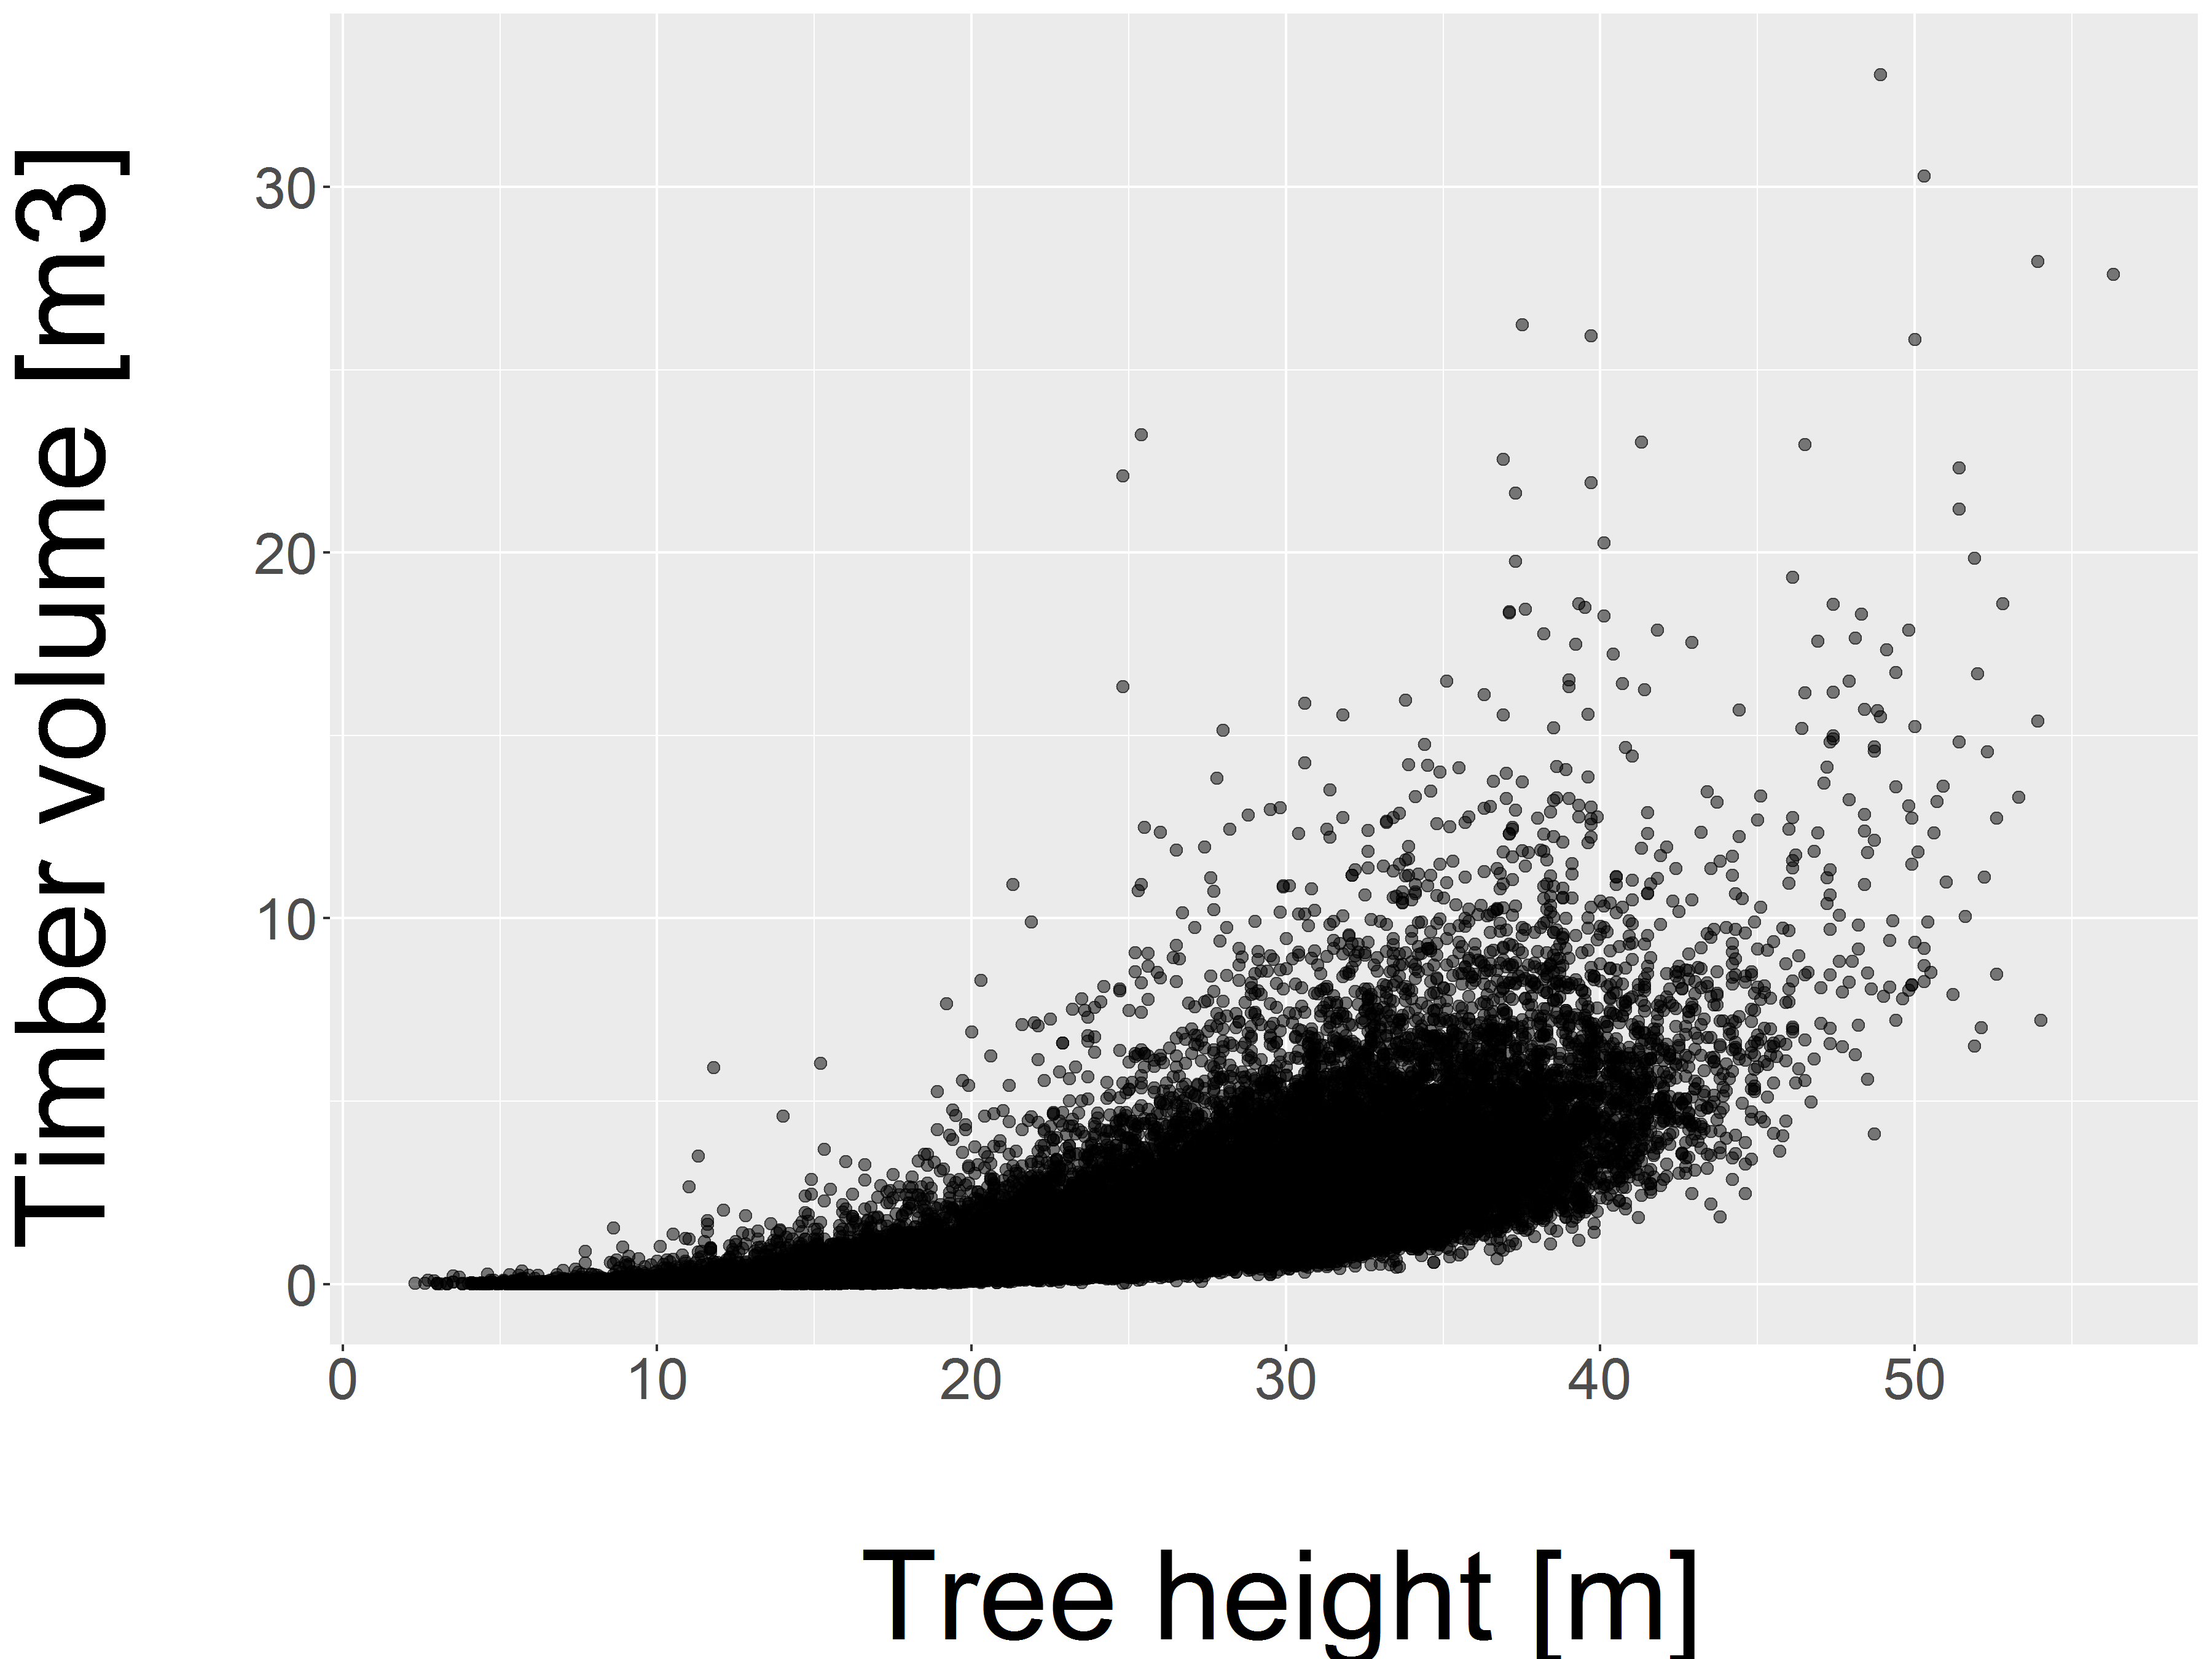
\includegraphics[width=0.6\textwidth]{fig/volr_vs_height_trees.png}%
  }\par\medskip
\subcaptionbox{Timber volume of sample trees plotted against tree height and tree species used in the \bwi{} taper functions}{
  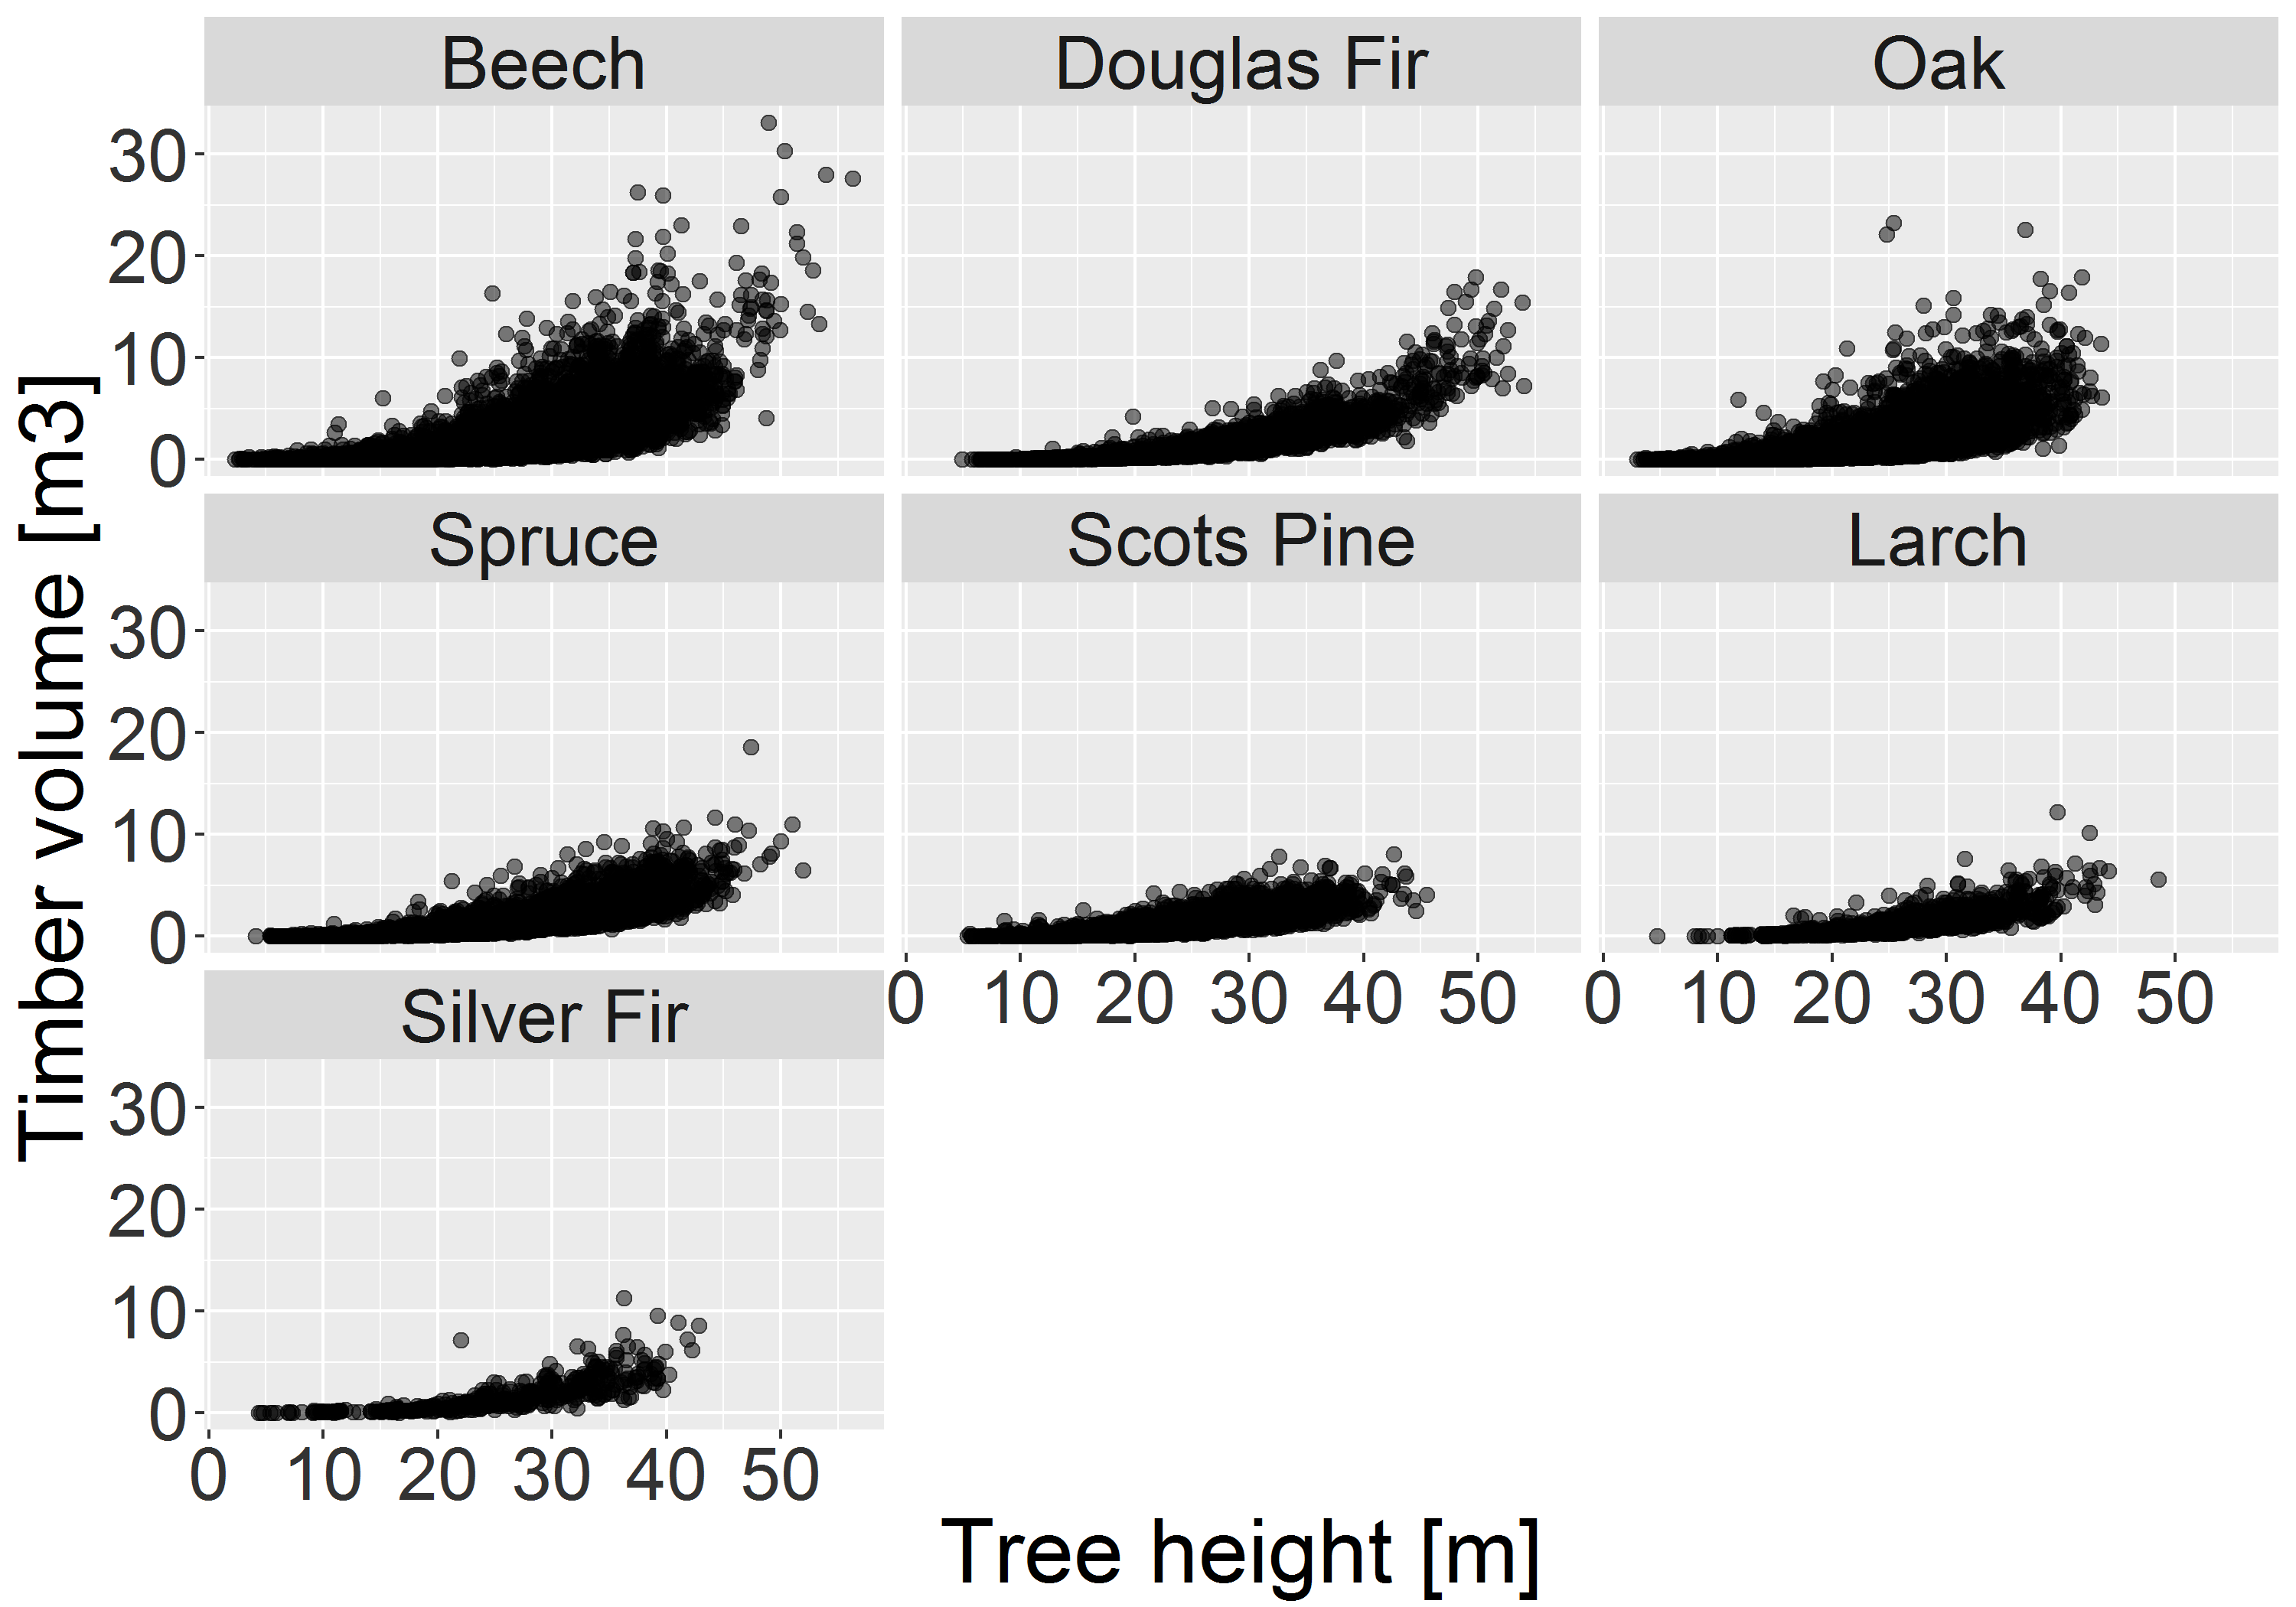
\includegraphics[width=0.7\textwidth]{fig/volr_vs_hoehe_ba_tarif.png}
  }\par\medskip
\caption{Timber volume relationships on single tree level of all \bwi{} sample trees within RLP}
\label{fig:rel_terr}
\end{figure}
\vfill

\newpage

% ----------------------------------------------------------------------- %
% 2 
% ----------------------------------------------------------------------- %


\textbf{\large 2: Timber volume on plot level vs. predictor variables}

\begin{figure}[H]
\centering
\subcaptionbox{Timber volume on plot level vs. LiDAR \textit{meanheight} stratified by the error-free \textit{treespecies} variable}{
  \includegraphics[width=0.8\textwidth]{fig/true_species.png}%
  }\par\medskip
\subcaptionbox{Timber volume on plot level vs. LiDAR \textit{meanheight} stratified by calibrated \textit{treespecies} variable}{
  \includegraphics[width=0.8\textwidth]{fig/calibrated_species.png}
  }\par\medskip
\caption{Timber volume on sample plot level stratified by the \textit{lidaryears} and \textit{treespecies}}
\label{fig:tvol_vs_lyear_tspec}
\end{figure}


% ----------------------------------------------------------------------- %
% 3
% ----------------------------------------------------------------------- %

\textbf{\large 3: Classification accuracies of $treespecies$ variable}
% latex table generated in R 3.4.2 by xtable 1.8-2 package
% Sat Jan 06 15:10:30 2018
\begingroup\fontsize{9pt}{10pt}\selectfont
\begin{longtable}{lllrrrrrrr}
	\caption{User's accuracies realized under various support choices for deriving 
		the major tree species of a sample location. $class$: major tree species class of 
		sample plot,
		$prod.acc$: producer's accuarcy, $use.acc$: user's accuracy, $oaa$: overall accuracy,
		$prod.acc_{cal}$: producer's accuarcy after calibration (use.acc and oaa respectively),
		$n.ref$: number of validation data per tree species.}\\ \\
	\hline
	class & support & threshold & prod.acc & $prod.acc_{cal}$ & use.acc & $use.acc_{cal}$ & oaa & $oaa_{cal}$ & n.ref \\ 
	\hline
	\endfirsthead
	\hline
	class & support & threshold & prod.acc & $prod.acc_{cal}$ & use.acc & $use.acc_{cal}$ & oaa & $oaa_{cal}$ & n.ref \\ 
	\hline
	\endhead
	\hline
	\multicolumn{10}{l}{\footnotesize Continued on next page}
	\endfoot
	\endlastfoot
Beech & ind & 0\% & 51.00 & 69.95 & 66.36 & 58.02 & 52.20 & 56.67 & 1857 \\ 
  Douglas Fir & ind & 0\% & 54.66 & 44.33 & 43.75 & 50.00 & 52.20 & 56.67 & 397 \\ 
  Oak & ind & 0\% & 65.53 & 39.20 & 41.67 & 47.57 & 52.20 & 56.67 & 824 \\ 
  Spruce & ind & 0\% & 58.92 & 68.66 & 64.38 & 62.35 & 52.20 & 56.67 & 1037 \\ 
  Scots pine & ind & 0\% & 67.45 & 62.06 & 45.51 & 59.93 & 52.20 & 56.67 & 593 \\ 
  Mixed & ind & 0\% & 2.87 & 16.48 & 8.20 & 42.16 & 52.20 & 56.67 & 522 \\ 
  Beech & ind & 50\% & 51.60 & 69.30 & 64.14 & 55.93 & 50.31 & 54.07 & 1723 \\ 
  Douglas Fir & ind & 50\% & 56.45 & 45.97 & 44.21 & 49.71 & 50.31 & 54.07 & 372 \\ 
  Oak & ind & 50\% & 66.24 & 39.95 & 40.70 & 46.90 & 50.31 & 54.07 & 776 \\ 
  Spruce & ind & 50\% & 58.87 & 67.64 & 63.48 & 60.83 & 50.31 & 54.07 & 992 \\ 
  Scots pine & ind & 50\% & 67.95 & 60.44 & 44.32 & 59.67 & 50.31 & 54.07 & 546 \\ 
  Mixed & ind & 50\% & 7.67 & 18.51 & 18.05 & 35.02 & 50.31 & 54.07 & 821 \\ 
  Beech & ind & 60\% & 48.56 & 68.79 & 62.12 & 54.52 & 47.55 & 52.33 & 1631 \\ 
  Douglas Fir & ind & 60\% & 53.74 & 43.49 & 44.29 & 47.29 & 47.55 & 52.33 & 361 \\ 
  Oak & ind & 60\% & 64.20 & 39.51 & 39.56 & 46.15 & 47.55 & 52.33 & 729 \\ 
  Spruce & ind & 60\% & 57.90 & 68.19 & 63.95 & 61.54 & 47.55 & 52.33 & 962 \\ 
  Scots pine & ind & 60\% & 66.53 & 55.92 & 41.69 & 58.17 & 47.55 & 52.33 & 490 \\ 
  Mixed & ind & 60\% & 14.19 & 22.71 & 22.03 & 35.35 & 47.55 & 52.33 & 1057 \\ 
  Beech & ind & 80\% & 44.16 & 37.47 & 50.15 & 50.24 & 45.45 & 53.77 & 1121 \\ 
  Douglas Fir & ind & 80\% & 48.32 & 37.25 & 42.99 & 48.47 & 45.45 & 53.77 & 298 \\ 
  Oak & ind & 80\% & 63.61 & 21.45 & 28.06 & 40.45 & 45.45 & 53.77 & 415 \\ 
  Spruce & ind & 80\% & 54.70 & 61.17 & 60.70 & 64.78 & 45.45 & 53.77 & 788 \\ 
  Scots pine & ind & 80\% & 65.70 & 35.74 & 30.33 & 55.00 & 45.45 & 53.77 & 277 \\ 
  Mixed & ind & 80\% & 36.94 & 69.11 & 51.96 & 53.33 & 45.45 & 53.77 & 2331 \\ 
  Beech & ind & 100\% & 38.58 & 19.90 & 41.42 & 48.80 & 50.82 & 63.86 & 819 \\ 
  Douglas Fir & ind & 100\% & 46.70 & 23.35 & 38.13 & 49.53 & 50.82 & 63.86 & 227 \\ 
  Oak & ind & 100\% & 61.69 & 10.73 & 21.73 & 40.00 & 50.82 & 63.86 & 261 \\ 
  Spruce & ind & 100\% & 50.86 & 49.45 & 55.38 & 65.22 & 50.82 & 63.86 & 637 \\ 
  Scots pine & ind & 100\% & 60.11 & 22.47 & 22.96 & 50.00 & 50.82 & 63.86 & 178 \\ 
  Mixed & ind & 100\% & 52.90 & 88.19 & 68.59 & 65.95 & 50.82 & 63.86 & 3108 \\ 
  Beech & q25 & 0\% & 50.03 & 72.02 & 66.99 & 58.83 & 52.14 & 56.88 & 1919 \\ 
  Douglas Fir & q25 & 0\% & 55.36 & 43.39 & 42.37 & 50.00 & 52.14 & 56.88 & 401 \\ 
  Oak & q25 & 0\% & 65.69 & 40.49 & 41.77 & 49.22 & 52.14 & 56.88 & 857 \\ 
  Spruce & q25 & 0\% & 59.16 & 67.75 & 63.85 & 61.42 & 52.14 & 56.88 & 1048 \\ 
  Scots pine & q25 & 0\% & 68.35 & 61.11 & 45.52 & 59.51 & 52.14 & 56.88 & 594 \\ 
  Mixed & q25 & 0\% & 3.75 & 12.92 & 10.81 & 37.30 & 52.14 & 56.88 & 534 \\ 
  Beech & q25 & 50\% & 51.07 & 73.54 & 65.07 & 56.94 & 50.36 & 55.56 & 1784 \\ 
  Douglas Fir & q25 & 50\% & 56.65 & 46.54 & 42.43 & 49.72 & 50.36 & 55.56 & 376 \\ 
  Oak & q25 & 50\% & 66.38 & 40.17 & 40.53 & 50.00 & 50.36 & 55.56 & 809 \\ 
  Spruce & q25 & 50\% & 59.80 & 69.45 & 63.40 & 61.44 & 50.36 & 55.56 & 1005 \\ 
  Scots pine & q25 & 50\% & 68.74 & 60.88 & 43.87 & 60.22 & 50.36 & 55.56 & 547 \\ 
  Mixed & q25 & 50\% & 6.97 & 15.75 & 18.07 & 36.59 & 50.36 & 55.56 & 832 \\ 
  Beech & q25 & 60\% & 49.62 & 72.71 & 62.27 & 54.04 & 47.97 & 52.55 & 1693 \\ 
  Douglas Fir & q25 & 60\% & 55.07 & 41.92 & 42.49 & 47.96 & 47.97 & 52.55 & 365 \\ 
  Oak & q25 & 60\% & 65.49 & 36.35 & 38.77 & 47.59 & 47.97 & 52.55 & 762 \\ 
  Spruce & q25 & 60\% & 59.49 & 68.51 & 63.46 & 59.86 & 47.97 & 52.55 & 975 \\ 
  Scots pine & q25 & 60\% & 68.02 & 56.62 & 40.78 & 59.53 & 47.97 & 52.55 & 491 \\ 
  Mixed & q25 & 60\% & 10.68 & 19.31 & 22.31 & 34.86 & 47.97 & 52.55 & 1067 \\ 
  Beech & q25 & 80\% & 43.39 & 36.95 & 50.05 & 47.86 & 43.98 & 51.93 & 1180 \\ 
  Douglas Fir & q25 & 80\% & 48.01 & 36.75 & 42.27 & 54.41 & 43.98 & 51.93 & 302 \\ 
  Oak & q25 & 80\% & 63.12 & 22.40 & 27.79 & 40.74 & 43.98 & 51.93 & 442 \\ 
  Spruce & q25 & 80\% & 55.12 & 62.25 & 60.66 & 62.09 & 43.98 & 51.93 & 800 \\ 
  Scots pine & q25 & 80\% & 65.11 & 35.97 & 29.05 & 55.25 & 43.98 & 51.93 & 278 \\ 
  Mixed & q25 & 80\% & 33.86 & 65.33 & 48.74 & 51.00 & 43.98 & 51.93 & 2351 \\ 
  Beech & q25 & 100\% & 36.72 & 16.42 & 41.55 & 48.81 & 48.65 & 62.58 & 877 \\ 
  Douglas Fir & q25 & 100\% & 42.17 & 21.74 & 40.25 & 48.54 & 48.65 & 62.58 & 230 \\ 
  Oak & q25 & 100\% & 57.14 & 8.01 & 20.53 & 46.94 & 48.65 & 62.58 & 287 \\ 
  Spruce & q25 & 100\% & 52.16 & 54.17 & 56.05 & 62.68 & 48.65 & 62.58 & 648 \\ 
  Scots pine & q25 & 100\% & 60.34 & 20.67 & 22.69 & 60.66 & 48.65 & 62.58 & 179 \\ 
  Mixed & q25 & 100\% & 50.29 & 87.64 & 64.05 & 64.06 & 48.65 & 62.58 & 3132 \\ 
  Beech & q50 & 0\% & 50.75 & 73.17 & 67.31 & 59.42 & 52.89 & 58.36 & 1931 \\ 
  Douglas Fir & q50 & 0\% & 54.98 & 47.01 & 42.02 & 56.08 & 52.89 & 58.36 & 402 \\ 
  Oak & q50 & 0\% & 67.44 & 43.49 & 41.76 & 52.31 & 52.89 & 58.36 & 860 \\ 
  Spruce & q50 & 0\% & 59.83 & 68.38 & 64.95 & 63.21 & 52.89 & 58.36 & 1053 \\ 
  Scots pine & q50 & 0\% & 70.25 & 62.86 & 45.39 & 59.37 & 52.89 & 58.36 & 595 \\ 
  Mixed & q50 & 0\% & 2.80 & 12.69 & 13.04 & 38.20 & 52.89 & 58.36 & 536 \\ 
  Beech & q50 & 50\% & 51.28 & 73.39 & 65.60 & 57.96 & 50.85 & 55.81 & 1796 \\ 
  Douglas Fir & q50 & 50\% & 55.17 & 47.48 & 42.80 & 53.92 & 50.85 & 55.81 & 377 \\ 
  Oak & q50 & 50\% & 67.36 & 44.83 & 40.85 & 52.53 & 50.85 & 55.81 & 812 \\ 
  Spruce & q50 & 50\% & 60.12 & 69.15 & 64.81 & 62.12 & 50.85 & 55.81 & 1008 \\ 
  Scots pine & q50 & 50\% & 70.44 & 58.58 & 44.99 & 57.42 & 50.85 & 55.81 & 548 \\ 
  Mixed & q50 & 50\% & 7.89 & 14.59 & 18.59 & 30.73 & 50.85 & 55.81 & 836 \\ 
  Beech & q50 & 60\% & 48.47 & 69.84 & 64.63 & 55.79 & 48.58 & 53.45 & 1704 \\ 
  Douglas Fir & q50 & 60\% & 51.91 & 44.26 & 45.56 & 51.59 & 48.58 & 53.45 & 366 \\ 
  Oak & q50 & 60\% & 64.31 & 45.75 & 40.13 & 50.58 & 48.58 & 53.45 & 765 \\ 
  Spruce & q50 & 60\% & 58.18 & 69.33 & 66.32 & 63.25 & 48.58 & 53.45 & 978 \\ 
  Scots pine & q50 & 60\% & 67.48 & 55.89 & 43.12 & 56.47 & 48.58 & 53.45 & 492 \\ 
  Mixed & q50 & 60\% & 18.94 & 20.43 & 24.52 & 32.25 & 48.58 & 53.45 & 1072 \\ 
  Beech & q50 & 80\% & 40.91 & 43.69 & 53.00 & 52.11 & 46.48 & 54.34 & 1188 \\ 
  Douglas Fir & q50 & 80\% & 45.21 & 39.27 & 48.07 & 60.10 & 46.48 & 54.34 & 303 \\ 
  Oak & q50 & 80\% & 60.67 & 24.04 & 29.61 & 39.78 & 46.48 & 54.34 & 445 \\ 
  Spruce & q50 & 80\% & 52.18 & 62.39 & 63.20 & 63.66 & 46.48 & 54.34 & 803 \\ 
  Scots pine & q50 & 80\% & 62.95 & 41.37 & 31.59 & 62.50 & 46.48 & 54.34 & 278 \\ 
  Mixed & q50 & 80\% & 42.88 & 66.14 & 49.46 & 53.04 & 46.48 & 54.34 & 2360 \\ 
  Beech & q50 & 100\% & 30.39 & 20.75 & 45.58 & 46.10 & 53.58 & 61.82 & 882 \\ 
  Douglas Fir & q50 & 100\% & 35.22 & 21.74 & 46.29 & 44.25 & 53.58 & 61.82 & 230 \\ 
  Oak & q50 & 100\% & 49.65 & 11.46 & 23.25 & 44.00 & 53.58 & 61.82 & 288 \\ 
  Spruce & q50 & 100\% & 43.47 & 53.61 & 58.11 & 60.70 & 53.58 & 61.82 & 651 \\ 
  Scots pine & q50 & 100\% & 58.10 & 26.26 & 28.42 & 52.22 & 53.58 & 61.82 & 179 \\ 
  Mixed & q50 & 100\% & 63.62 & 84.59 & 63.64 & 64.50 & 53.58 & 61.82 & 3147 \\ 
  Beech & q80 & 0\% & 51.16 & 73.41 & 67.05 & 59.67 & 53.33 & 58.52 & 1937 \\ 
  Douglas Fir & q80 & 0\% & 55.45 & 47.52 & 42.83 & 56.80 & 53.33 & 58.52 & 404 \\ 
  Oak & q80 & 0\% & 67.82 & 43.75 & 41.74 & 52.07 & 53.33 & 58.52 & 864 \\ 
  Spruce & q80 & 0\% & 60.95 & 68.63 & 65.75 & 63.34 & 53.33 & 58.52 & 1055 \\ 
  Scots pine & q80 & 0\% & 71.19 & 60.97 & 45.95 & 58.43 & 53.33 & 58.52 & 597 \\ 
  Mixed & q80 & 0\% & 2.03 & 14.73 & 11.96 & 42.78 & 53.33 & 58.52 & 543 \\ 
  Beech & q80 & 50\% & 51.17 & 72.42 & 66.05 & 57.90 & 51.70 & 56.06 & 1802 \\ 
  Douglas Fir & q80 & 50\% & 55.94 & 46.44 & 45.11 & 53.99 & 51.70 & 56.06 & 379 \\ 
  Oak & q80 & 50\% & 67.52 & 45.10 & 41.43 & 51.90 & 51.70 & 56.06 & 816 \\ 
  Spruce & q80 & 50\% & 60.99 & 69.50 & 66.17 & 62.46 & 51.70 & 56.06 & 1010 \\ 
  Scots pine & q80 & 50\% & 70.67 & 59.20 & 46.75 & 59.74 & 51.70 & 56.06 & 549 \\ 
  Mixed & q80 & 50\% & 12.20 & 17.89 & 23.25 & 34.09 & 51.70 & 56.06 & 844 \\ 
  Beech & q80 & 60\% & 47.25 & 70.23 & 65.69 & 56.78 & 48.76 & 54.59 & 1710 \\ 
  Douglas Fir & q80 & 60\% & 51.90 & 46.47 & 49.61 & 52.29 & 48.76 & 54.59 & 368 \\ 
  Oak & q80 & 60\% & 63.98 & 47.33 & 41.80 & 49.66 & 48.76 & 54.59 & 769 \\ 
  Spruce & q80 & 60\% & 56.94 & 69.59 & 67.55 & 63.44 & 48.76 & 54.59 & 980 \\ 
  Scots pine & q80 & 60\% & 66.53 & 55.58 & 44.99 & 60.22 & 48.76 & 54.59 & 493 \\ 
  Mixed & q80 & 60\% & 23.70 & 23.70 & 24.31 & 36.83 & 48.76 & 54.59 & 1080 \\ 
  Beech & q80 & 80\% & 37.80 & 39.90 & 55.68 & 51.63 & 47.91 & 53.67 & 1193 \\ 
  Douglas Fir & q80 & 80\% & 40.33 & 37.70 & 51.46 & 60.21 & 47.91 & 53.67 & 305 \\ 
  Oak & q80 & 80\% & 57.49 & 25.73 & 30.85 & 41.52 & 47.91 & 53.67 & 447 \\ 
  Spruce & q80 & 80\% & 49.00 & 60.57 & 64.27 & 63.99 & 47.91 & 53.67 & 804 \\ 
  Scots pine & q80 & 80\% & 62.01 & 40.86 & 35.97 & 66.28 & 47.91 & 53.67 & 279 \\ 
  Mixed & q80 & 80\% & 50.13 & 67.07 & 49.05 & 51.71 & 47.91 & 53.67 & 2372 \\ 
  Beech & q80 & 100\% & 25.54 & 22.94 & 50.45 & 49.88 & 57.41 & 62.61 & 885 \\ 
  Douglas Fir & q80 & 100\% & 29.13 & 23.91 & 53.17 & 52.88 & 57.41 & 62.61 & 230 \\ 
  Oak & q80 & 100\% & 40.83 & 13.49 & 25.76 & 52.70 & 57.41 & 62.61 & 289 \\ 
  Spruce & q80 & 100\% & 36.96 & 48.16 & 61.95 & 60.15 & 57.41 & 62.61 & 652 \\ 
  Scots pine & q80 & 100\% & 51.67 & 30.00 & 34.19 & 60.00 & 57.41 & 62.61 & 180 \\ 
  Mixed & q80 & 100\% & 74.43 & 85.84 & 63.53 & 64.62 & 57.41 & 62.61 & 3164 \\ 
  Beech & q100 & 0\% & 53.73 & 72.96 & 67.46 & 59.55 & 55.24 & 58.53 & 1945 \\ 
  Douglas Fir & q100 & 0\% & 55.88 & 47.30 & 45.97 & 54.21 & 55.24 & 58.53 & 408 \\ 
  Oak & q100 & 0\% & 71.35 & 47.18 & 43.27 & 53.25 & 55.24 & 58.53 & 869 \\ 
  Spruce & q100 & 0\% & 62.70 & 66.29 & 66.14 & 63.02 & 55.24 & 58.53 & 1059 \\ 
  Scots pine & q100 & 0\% & 73.83 & 65.67 & 46.98 & 63.14 & 55.24 & 58.53 & 600 \\ 
  Mixed & q100 & 0\% & 0.18 & 11.23 & 12.50 & 33.33 & 55.24 & 58.53 & 552 \\ 
  Beech & q100 & 50\% & 48.45 & 71.66 & 68.95 & 57.49 & 51.87 & 56.27 & 1810 \\ 
  Douglas Fir & q100 & 50\% & 49.74 & 48.69 & 55.39 & 56.02 & 51.87 & 56.27 & 382 \\ 
  Oak & q100 & 50\% & 68.21 & 49.45 & 46.40 & 53.63 & 51.87 & 56.27 & 821 \\ 
  Spruce & q100 & 50\% & 57.69 & 67.85 & 68.74 & 62.77 & 51.87 & 56.27 & 1014 \\ 
  Scots pine & q100 & 50\% & 68.78 & 63.70 & 54.85 & 61.69 & 51.87 & 56.27 & 551 \\ 
  Mixed & q100 & 50\% & 26.55 & 15.09 & 21.23 & 30.50 & 51.87 & 56.27 & 855 \\ 
  Beech & q100 & 60\% & 40.98 & 68.45 & 69.02 & 55.84 & 48.56 & 52.81 & 1718 \\ 
  Douglas Fir & q100 & 60\% & 40.70 & 42.86 & 57.85 & 51.79 & 48.56 & 52.81 & 371 \\ 
  Oak & q100 & 60\% & 61.24 & 46.64 & 48.12 & 50.35 & 48.56 & 52.81 & 774 \\ 
  Spruce & q100 & 60\% & 51.12 & 67.78 & 70.75 & 61.93 & 48.56 & 52.81 & 984 \\ 
  Scots pine & q100 & 60\% & 63.03 & 58.18 & 57.78 & 60.00 & 48.56 & 52.81 & 495 \\ 
  Mixed & q100 & 60\% & 45.28 & 19.98 & 25.78 & 29.22 & 48.56 & 52.81 & 1091 \\ 
  Beech & q100 & 80\% & 27.55 & 40.15 & 63.22 & 51.06 & 51.15 & 53.49 & 1198 \\ 
  Douglas Fir & q100 & 80\% & 26.30 & 28.57 & 63.78 & 58.67 & 51.15 & 53.49 & 308 \\ 
  Oak & q100 & 80\% & 47.12 & 26.55 & 36.47 & 44.12 & 51.15 & 53.49 & 452 \\ 
  Spruce & q100 & 80\% & 36.80 & 60.35 & 69.72 & 62.92 & 51.15 & 53.49 & 807 \\ 
  Scots pine & q100 & 80\% & 57.35 & 44.09 & 52.29 & 64.06 & 51.15 & 53.49 & 279 \\ 
  Mixed & q100 & 80\% & 71.08 & 67.27 & 48.96 & 51.79 & 51.15 & 53.49 & 2389 \\ 
  Beech & q100 & 100\% & 5.29 & 19.69 & 55.29 & 40.98 & 59.36 & 59.51 & 889 \\ 
  Douglas Fir & q100 & 100\% & 7.79 & 10.39 & 69.23 & 40.68 & 59.36 & 59.51 & 231 \\ 
  Oak & q100 & 100\% & 11.26 & 7.85 & 27.73 & 30.26 & 59.36 & 59.51 & 293 \\ 
  Spruce & q100 & 100\% & 11.81 & 43.87 & 77.78 & 52.87 & 59.36 & 59.51 & 652 \\ 
  Scots pine & q100 & 100\% & 20.56 & 25.00 & 50.68 & 52.94 & 59.36 & 59.51 & 180 \\ 
  Mixed & q100 & 100\% & 94.51 & 84.07 & 59.89 & 63.13 & 59.36 & 59.51 & 3188 \\ 
  \hline
\end{longtable}
\endgroup\newpage



% ----------------------------------------------------------------------- %
% 4 & 5
% ----------------------------------------------------------------------- %

\textbf{\large 4: Model accuracies}\\

% latex table generated in R 3.3.2 by xtable 1.8-2 package
% Tue Apr 25 10:42:03 2017
\begingroup\fontsize{9pt}{10pt}\selectfont
\begin{longtable}{lllrrrrrr}
\caption{Model accuracies realized under various 
                       support choices for the CHM- and \textbf{uncalibrated} $treespecies$ 
                       explanatory variables}\\ \\
\hline
$support_{chm}$ & $support_{tspec}$ & threshold & $R^2_{adj}$ & $rmse_{cv}$ & AIC & $R^2_{adj, ref}$ & $rmse_{cv, ref}$ & $AIC_{ref}$ \\ 
  \hline
\endfirsthead
  \hline
$support_{chm}$ & $support_{tspec}$ & threshold & $R^2_{adj}$ & $rmse_{cv}$ & AIC & $R^2_{adj, ref}$ & $rmse_{cv, ref}$ & $AIC_{ref}$ \\ 
  \hline
\endhead
\hline
\multicolumn{9}{l}{\footnotesize Continued on next page}
\endfoot
\endlastfoot
ind & ind & 0\% & 0.45 & 135.49 & 64565.00 & 0.47 & 133.56 & 64565.00 \\ 
  ind & ind & 50\% & 0.45 & 135.57 & 64569.96 & 0.47 & 133.80 & 64569.96 \\ 
  ind & ind & 60\% & 0.45 & 135.52 & 64564.50 & 0.47 & 133.73 & 64564.50 \\ 
  ind & ind & 80\% & 0.46 & 135.26 & 64551.18 & 0.47 & 133.44 & 64551.18 \\ 
  ind & ind & 100\% & 0.45 & 135.65 & 64584.58 & 0.47 & 133.03 & 64584.58 \\ 
  ind & q25 & 0\% & 0.46 & 135.37 & 64912.94 & 0.47 & 133.46 & 64912.94 \\ 
  ind & q25 & 50\% & 0.46 & 135.22 & 64899.31 & 0.47 & 133.81 & 64899.31 \\ 
  ind & q25 & 60\% & 0.46 & 135.07 & 64895.72 & 0.47 & 133.85 & 64895.72 \\ 
  ind & q25 & 80\% & 0.46 & 135.27 & 64896.97 & 0.47 & 133.36 & 64896.97 \\ 
  ind & q25 & 100\% & 0.46 & 135.42 & 64920.27 & 0.48 & 133.02 & 64920.27 \\ 
  ind & q50 & 0\% & 0.46 & 135.54 & 65166.10 & 0.47 & 133.61 & 65166.10 \\ 
  ind & q50 & 50\% & 0.46 & 135.52 & 65157.65 & 0.47 & 133.79 & 65157.65 \\ 
  ind & q50 & 60\% & 0.46 & 135.54 & 65168.94 & 0.47 & 133.68 & 65168.94 \\ 
  ind & q50 & 80\% & 0.46 & 135.35 & 65150.63 & 0.47 & 133.32 & 65150.63 \\ 
  ind & q50 & 100\% & 0.46 & 135.57 & 65168.81 & 0.48 & 132.93 & 65168.81 \\ 
  ind & q80 & 0\% & 0.46 & 135.44 & 65389.21 & 0.47 & 133.50 & 65389.21 \\ 
  ind & q80 & 50\% & 0.46 & 135.13 & 65367.67 & 0.47 & 133.87 & 65367.67 \\ 
  ind & q80 & 60\% & 0.46 & 135.21 & 65376.26 & 0.47 & 133.87 & 65376.26 \\ 
  ind & q80 & 80\% & 0.46 & 135.21 & 65384.06 & 0.47 & 133.44 & 65384.06 \\ 
  ind & q80 & 100\% & 0.45 & 136.59 & 65489.16 & 0.48 & 132.98 & 65489.16 \\ 
  ind & q100 & 0\% & 0.46 & 135.32 & 65722.46 & 0.47 & 133.45 & 65722.46 \\ 
  ind & q100 & 50\% & 0.46 & 135.32 & 65699.46 & 0.47 & 133.75 & 65699.46 \\ 
  ind & q100 & 60\% & 0.46 & 135.67 & 65728.34 & 0.47 & 133.69 & 65728.34 \\ 
  ind & q100 & 80\% & 0.45 & 136.66 & 65813.95 & 0.47 & 133.32 & 65813.95 \\ 
  ind & q100 & 100\% & 0.44 & 137.78 & 65919.21 & 0.48 & 132.91 & 65919.21 \\ 
  q25 & ind & 0\% & 0.46 & 135.53 & 64882.32 & 0.47 & 133.73 & 64882.32 \\ 
  q25 & ind & 50\% & 0.46 & 135.63 & 64886.16 & 0.47 & 134.07 & 64886.16 \\ 
  q25 & ind & 60\% & 0.46 & 135.58 & 64881.59 & 0.47 & 134.02 & 64881.59 \\ 
  q25 & ind & 80\% & 0.46 & 135.40 & 64869.18 & 0.48 & 133.58 & 64869.18 \\ 
  q25 & ind & 100\% & 0.46 & 135.58 & 64888.87 & 0.48 & 133.13 & 64888.87 \\ 
  q25 & q25 & 0\% & 0.47 & 135.42 & 65600.99 & 0.48 & 133.37 & 65600.99 \\ 
  q25 & q25 & 50\% & 0.47 & 135.24 & 65590.23 & 0.48 & 133.76 & 65590.23 \\ 
  q25 & q25 & 60\% & 0.47 & 135.20 & 65586.93 & 0.48 & 133.71 & 65586.93 \\ 
  q25 & q25 & 80\% & 0.47 & 135.21 & 65589.23 & 0.48 & 133.39 & 65589.23 \\ 
  q25 & q25 & 100\% & 0.47 & 135.55 & 65616.63 & 0.49 & 132.97 & 65616.63 \\ 
  q25 & q50 & 0\% & 0.47 & 135.02 & 65848.23 & 0.48 & 133.19 & 65848.23 \\ 
  q25 & q50 & 50\% & 0.47 & 135.00 & 65842.32 & 0.48 & 133.40 & 65842.32 \\ 
  q25 & q50 & 60\% & 0.46 & 135.28 & 65860.37 & 0.48 & 133.31 & 65860.37 \\ 
  q25 & q50 & 80\% & 0.47 & 134.98 & 65839.14 & 0.48 & 133.00 & 65839.14 \\ 
  q25 & q50 & 100\% & 0.46 & 135.27 & 65864.46 & 0.49 & 132.40 & 65864.46 \\ 
  q25 & q80 & 0\% & 0.47 & 135.20 & 66065.23 & 0.48 & 133.26 & 66065.23 \\ 
  q25 & q80 & 50\% & 0.47 & 134.93 & 66048.51 & 0.48 & 133.55 & 66048.51 \\ 
  q25 & q80 & 60\% & 0.47 & 134.98 & 66059.78 & 0.48 & 133.53 & 66059.78 \\ 
  q25 & q80 & 80\% & 0.47 & 135.19 & 66072.89 & 0.48 & 133.18 & 66072.89 \\ 
  q25 & q80 & 100\% & 0.46 & 136.38 & 66178.69 & 0.49 & 132.75 & 66178.69 \\ 
  q25 & q100 & 0\% & 0.47 & 143.40 & 66410.21 & 0.48 & 133.13 & 66410.21 \\ 
  q25 & q100 & 50\% & 0.47 & 134.73 & 66384.24 & 0.48 & 133.39 & 66384.24 \\ 
  q25 & q100 & 60\% & 0.47 & 135.23 & 66419.67 & 0.48 & 133.41 & 66419.67 \\ 
  q25 & q100 & 80\% & 0.46 & 136.36 & 66511.85 & 0.48 & 133.01 & 66511.85 \\ 
  q25 & q100 & 100\% & 0.45 & 137.67 & 66621.81 & 0.49 & 132.58 & 66621.81 \\ 
  q50 & ind & 0\% & 0.46 & 135.13 & 64847.79 & 0.48 & 133.11 & 64847.79 \\ 
  q50 & ind & 50\% & 0.46 & 135.24 & 64851.64 & 0.48 & 133.44 & 64851.64 \\ 
  q50 & ind & 60\% & 0.46 & 135.22 & 64847.03 & 0.48 & 133.43 & 64847.03 \\ 
  q50 & ind & 80\% & 0.46 & 134.96 & 64831.38 & 0.48 & 133.11 & 64831.38 \\ 
  q50 & ind & 100\% & 0.46 & 135.26 & 64862.89 & 0.48 & 132.62 & 64862.89 \\ 
  q50 & q25 & 0\% & 0.47 & 134.80 & 65557.75 & 0.49 & 132.59 & 65557.75 \\ 
  q50 & q25 & 50\% & 0.47 & 134.61 & 65546.50 & 0.49 & 132.92 & 65546.50 \\ 
  q50 & q25 & 60\% & 0.47 & 134.57 & 65543.07 & 0.49 & 132.91 & 65543.07 \\ 
  q50 & q25 & 80\% & 0.47 & 134.51 & 65540.80 & 0.49 & 132.69 & 65540.80 \\ 
  q50 & q25 & 100\% & 0.47 & 134.92 & 65572.25 & 0.49 & 132.33 & 65572.25 \\ 
  q50 & q50 & 0\% & 0.47 & 134.37 & 65805.45 & 0.49 & 132.36 & 65805.45 \\ 
  q50 & q50 & 50\% & 0.47 & 134.34 & 65800.77 & 0.49 & 132.57 & 65800.77 \\ 
  q50 & q50 & 60\% & 0.47 & 134.53 & 65815.15 & 0.49 & 132.54 & 65815.15 \\ 
  q50 & q50 & 80\% & 0.47 & 134.21 & 65789.54 & 0.49 & 132.25 & 65789.54 \\ 
  q50 & q50 & 100\% & 0.47 & 134.66 & 65825.59 & 0.49 & 131.74 & 65825.59 \\ 
  q50 & q80 & 0\% & 0.47 & 134.57 & 66019.32 & 0.49 & 132.53 & 66019.32 \\ 
  q50 & q80 & 50\% & 0.47 & 134.36 & 66006.32 & 0.49 & 132.82 & 66006.32 \\ 
  q50 & q80 & 60\% & 0.47 & 134.41 & 66015.77 & 0.49 & 132.79 & 66015.77 \\ 
  q50 & q80 & 80\% & 0.47 & 134.57 & 66025.39 & 0.49 & 132.62 & 66025.39 \\ 
  q50 & q80 & 100\% & 0.46 & 135.80 & 66132.10 & 0.49 & 132.18 & 66132.10 \\ 
  q50 & q100 & 0\% & 0.47 & 137.56 & 66365.96 & 0.49 & 132.48 & 66365.96 \\ 
  q50 & q100 & 50\% & 0.47 & 134.21 & 66345.91 & 0.49 & 132.72 & 66345.91 \\ 
  q50 & q100 & 60\% & 0.47 & 134.69 & 66381.21 & 0.49 & 132.72 & 66381.21 \\ 
  q50 & q100 & 80\% & 0.46 & 135.78 & 66468.28 & 0.49 & 132.46 & 66468.28 \\ 
  q50 & q100 & 100\% & 0.45 & 137.06 & 66575.44 & 0.49 & 132.03 & 66575.44 \\ 
  q80 & ind & 0\% & 0.46 & 135.78 & 64898.36 & 0.47 & 133.82 & 64898.36 \\ 
  q80 & ind & 50\% & 0.46 & 135.90 & 64900.98 & 0.47 & 134.21 & 64900.98 \\ 
  q80 & ind & 60\% & 0.46 & 135.85 & 64895.77 & 0.47 & 134.20 & 64895.77 \\ 
  q80 & ind & 80\% & 0.46 & 135.70 & 64890.76 & 0.47 & 133.79 & 64890.76 \\ 
  q80 & ind & 100\% & 0.45 & 136.06 & 64925.51 & 0.48 & 133.26 & 64925.51 \\ 
  q80 & q25 & 0\% & 0.47 & 135.53 & 65611.68 & 0.48 & 133.44 & 65611.68 \\ 
  q80 & q25 & 50\% & 0.47 & 135.36 & 65600.46 & 0.48 & 133.78 & 65600.46 \\ 
  q80 & q25 & 60\% & 0.47 & 135.29 & 65595.97 & 0.48 & 133.76 & 65595.97 \\ 
  q80 & q25 & 80\% & 0.47 & 135.35 & 65599.65 & 0.48 & 133.53 & 65599.65 \\ 
  q80 & q25 & 100\% & 0.46 & 135.78 & 65634.33 & 0.49 & 133.04 & 65634.33 \\ 
  q80 & q50 & 0\% & 0.46 & 135.09 & 65860.84 & 0.48 & 133.11 & 65860.84 \\ 
  q80 & q50 & 50\% & 0.47 & 135.10 & 65857.40 & 0.48 & 133.40 & 65857.40 \\ 
  q80 & q50 & 60\% & 0.46 & 135.25 & 65869.26 & 0.48 & 133.39 & 65869.26 \\ 
  q80 & q50 & 80\% & 0.47 & 135.08 & 65857.71 & 0.48 & 133.06 & 65857.71 \\ 
  q80 & q50 & 100\% & 0.46 & 135.52 & 65890.97 & 0.49 & 132.45 & 65890.97 \\ 
  q80 & q80 & 0\% & 0.47 & 135.29 & 66078.42 & 0.48 & 133.27 & 66078.42 \\ 
  q80 & q80 & 50\% & 0.47 & 135.06 & 66063.08 & 0.48 & 133.60 & 66063.08 \\ 
  q80 & q80 & 60\% & 0.47 & 135.20 & 66077.30 & 0.48 & 133.60 & 66077.30 \\ 
  q80 & q80 & 80\% & 0.47 & 135.38 & 66089.20 & 0.48 & 133.33 & 66089.20 \\ 
  q80 & q80 & 100\% & 0.45 & 136.64 & 66197.34 & 0.49 & 132.82 & 66197.34 \\ 
  q80 & q100 & 0\% & 0.47 & 136.20 & 66438.48 & 0.48 & 133.22 & 66438.48 \\ 
  q80 & q100 & 50\% & 0.47 & 135.00 & 66413.28 & 0.48 & 133.51 & 66413.28 \\ 
  q80 & q100 & 60\% & 0.46 & 135.43 & 66445.71 & 0.48 & 133.51 & 66445.71 \\ 
  q80 & q100 & 80\% & 0.46 & 136.63 & 66538.24 & 0.48 & 133.16 & 66538.24 \\ 
  q80 & q100 & 100\% & 0.44 & 137.89 & 66642.87 & 0.49 & 132.64 & 66642.87 \\ 
  q100 & ind & 0\% & 0.39 & 143.82 & 65494.94 & 0.41 & 142.07 & 65494.94 \\ 
  q100 & ind & 50\% & 0.39 & 143.93 & 65496.27 & 0.40 & 142.38 & 65496.27 \\ 
  q100 & ind & 60\% & 0.39 & 143.83 & 65492.62 & 0.40 & 142.41 & 65492.62 \\ 
  q100 & ind & 80\% & 0.39 & 143.83 & 65494.72 & 0.41 & 142.00 & 65494.72 \\ 
  q100 & ind & 100\% & 0.39 & 143.98 & 65512.77 & 0.41 & 141.55 & 65512.77 \\ 
  q100 & q25 & 0\% & 0.40 & 143.88 & 66234.56 & 0.41 & 141.95 & 66234.56 \\ 
  q100 & q25 & 50\% & 0.40 & 143.64 & 66219.68 & 0.41 & 142.27 & 66219.68 \\ 
  q100 & q25 & 60\% & 0.40 & 143.56 & 66214.76 & 0.41 & 142.30 & 66214.76 \\ 
  q100 & q25 & 80\% & 0.40 & 143.77 & 66225.18 & 0.41 & 141.99 & 66225.18 \\ 
  q100 & q25 & 100\% & 0.40 & 144.09 & 66251.66 & 0.42 & 141.48 & 66251.66 \\ 
  q100 & q50 & 0\% & 0.40 & 143.49 & 66484.62 & 0.41 & 141.65 & 66484.62 \\ 
  q100 & q50 & 50\% & 0.40 & 143.52 & 66483.55 & 0.41 & 141.96 & 66483.55 \\ 
  q100 & q50 & 60\% & 0.40 & 143.69 & 66495.93 & 0.41 & 141.97 & 66495.93 \\ 
  q100 & q50 & 80\% & 0.40 & 143.62 & 66491.72 & 0.41 & 141.63 & 66491.72 \\ 
  q100 & q50 & 100\% & 0.39 & 143.87 & 66506.91 & 0.42 & 140.99 & 66506.91 \\ 
  q100 & q80 & 0\% & 0.40 & 143.60 & 66712.36 & 0.41 & 141.85 & 66712.36 \\ 
  q100 & q80 & 50\% & 0.40 & 143.35 & 66693.16 & 0.41 & 142.18 & 66693.16 \\ 
  q100 & q80 & 60\% & 0.40 & 143.66 & 66712.41 & 0.41 & 142.19 & 66712.41 \\ 
  q100 & q80 & 80\% & 0.40 & 143.86 & 66719.35 & 0.41 & 141.86 & 66719.35 \\ 
  q100 & q80 & 100\% & 0.39 & 145.04 & 66822.81 & 0.42 & 141.32 & 66822.81 \\ 
  q100 & q100 & 0\% & 0.39 & 145.21 & 67092.26 & 0.41 & 142.01 & 67092.26 \\ 
  q100 & q100 & 50\% & 0.40 & 143.61 & 67060.58 & 0.41 & 142.24 & 67060.58 \\ 
  q100 & q100 & 60\% & 0.40 & 144.01 & 67086.87 & 0.41 & 142.25 & 67086.87 \\ 
  q100 & q100 & 80\% & 0.39 & 145.17 & 67169.91 & 0.41 & 141.79 & 67169.91 \\ 
  q100 & q100 & 100\% & 0.37 & 146.66 & 67284.45 & 0.42 & 141.22 & 67284.45 \\ 
  \hline
\end{longtable}
\endgroup
\newpage

% latex table generated in R 3.4.2 by xtable 1.8-2 package
% Sun Jan 07 10:52:56 2018
\begingroup\fontsize{7pt}{8pt}\selectfont
\begin{longtable}{lllrrrrrrrr}
\caption{Model accuracies realized under various 
	support choices for the CHM- and \textbf{calibrated} $treespecies$ 
	explanatory variables}\\ \\
	\hline
	$support_{chm}$ & $support_{tspec}$ & $threshold$ & $R^2_{adj}$ & $RMSE_{cv}$ & $RMSE_{cv}[\%]$ & $AIC$ & $R^2_{adj, ref}$ & $RMSE_{cv, ref}$ & $RMSE_{cv, ref}[\%]$ & $AIC_{ref}$ \\ 
	\hline
	\endfirsthead
	\hline
	$support_{chm}$ & $support_{tspec}$ & $threshold$ & $R^2_{adj}$ & $RMSE_{cv}$ & $RMSE_{cv}[\%]$ & $AIC$ & $R^2_{adj, ref}$ & $RMSE_{cv, ref}$ & $RMSE_{cv, ref}[\%]$ & $AIC_{ref}$ \\ 
	\hline
	\endhead
	\hline
	\multicolumn{11}{l}{\footnotesize Continued on next page}
	\endfoot
	\endlastfoot
ind & ind & 0\% & 0.45 & 140.12 & 43.61 & 64291.15 & 0.45 & 139.71 & 43.48 & 64256.93 \\ 
  ind & ind & 50\% & 0.45 & 140.60 & 43.75 & 64317.74 & 0.45 & 139.85 & 43.52 & 64268.78 \\ 
  ind & ind & 60\% & 0.45 & 140.13 & 43.61 & 64294.65 & 0.45 & 139.48 & 43.41 & 64255.23 \\ 
  ind & ind & 80\% & 0.46 & 139.10 & 43.29 & 64236.04 & 0.46 & 138.92 & 43.23 & 64225.80 \\ 
  ind & ind & 100\% & 0.45 & 139.92 & 43.54 & 64280.23 & 0.46 & 138.85 & 43.21 & 64204.65 \\ 
  ind & q25 & 0\% & 0.45 & 139.90 & 43.97 & 64835.11 & 0.46 & 139.25 & 43.77 & 64780.23 \\ 
  ind & q25 & 50\% & 0.45 & 140.06 & 44.02 & 64852.35 & 0.46 & 139.37 & 43.81 & 64795.25 \\ 
  ind & q25 & 60\% & 0.45 & 139.97 & 43.99 & 64846.98 & 0.46 & 139.23 & 43.76 & 64783.04 \\ 
  ind & q25 & 80\% & 0.46 & 139.17 & 43.74 & 64792.34 & 0.46 & 138.57 & 43.56 & 64749.77 \\ 
  ind & q25 & 100\% & 0.46 & 139.16 & 43.74 & 64792.06 & 0.46 & 138.14 & 43.42 & 64725.81 \\ 
  ind & q50 & 0\% & 0.45 & 139.91 & 44.17 & 65093.04 & 0.46 & 139.36 & 44.00 & 65057.03 \\ 
  ind & q50 & 50\% & 0.45 & 140.25 & 44.28 & 65113.44 & 0.46 & 139.60 & 44.07 & 65072.06 \\ 
  ind & q50 & 60\% & 0.45 & 139.89 & 44.16 & 65094.92 & 0.46 & 139.53 & 44.05 & 65060.08 \\ 
  ind & q50 & 80\% & 0.46 & 139.02 & 43.89 & 65033.71 & 0.46 & 138.90 & 43.85 & 65026.35 \\ 
  ind & q50 & 100\% & 0.46 & 139.19 & 43.94 & 65040.22 & 0.46 & 138.60 & 43.75 & 65002.79 \\ 
  ind & q80 & 0\% & 0.46 & 139.68 & 44.24 & 65309.58 & 0.46 & 139.43 & 44.16 & 65282.95 \\ 
  ind & q80 & 50\% & 0.45 & 139.97 & 44.33 & 65336.21 & 0.46 & 139.71 & 44.25 & 65297.81 \\ 
  ind & q80 & 60\% & 0.46 & 139.97 & 44.33 & 65319.59 & 0.46 & 139.58 & 44.21 & 65286.72 \\ 
  ind & q80 & 80\% & 0.46 & 139.25 & 44.11 & 65283.08 & 0.46 & 138.97 & 44.02 & 65252.00 \\ 
  ind & q80 & 100\% & 0.46 & 139.09 & 44.05 & 65251.61 & 0.46 & 138.84 & 43.98 & 65227.79 \\ 
  ind & q100 & 0\% & 0.46 & 138.89 & 43.73 & 65577.54 & 0.46 & 138.83 & 43.72 & 65570.10 \\ 
  ind & q100 & 50\% & 0.46 & 139.18 & 43.82 & 65589.23 & 0.46 & 139.13 & 43.81 & 65585.38 \\ 
  ind & q100 & 60\% & 0.46 & 139.21 & 43.83 & 65580.00 & 0.46 & 139.14 & 43.81 & 65575.20 \\ 
  ind & q100 & 80\% & 0.46 & 138.43 & 43.59 & 65543.72 & 0.46 & 138.39 & 43.58 & 65541.28 \\ 
  ind & q100 & 100\% & 0.46 & 138.34 & 43.56 & 65521.67 & 0.46 & 138.25 & 43.53 & 65513.09 \\ 
  q25 & ind & 0\% & 0.45 & 140.80 & 44.04 & 64815.81 & 0.46 & 140.09 & 43.82 & 64776.64 \\ 
  q25 & ind & 50\% & 0.45 & 140.79 & 44.04 & 64815.82 & 0.46 & 140.28 & 43.88 & 64790.59 \\ 
  q25 & ind & 60\% & 0.45 & 140.73 & 44.02 & 64812.34 & 0.46 & 139.96 & 43.78 & 64778.10 \\ 
  q25 & ind & 80\% & 0.46 & 139.93 & 43.77 & 64780.19 & 0.46 & 139.43 & 43.62 & 64756.67 \\ 
  q25 & ind & 100\% & 0.45 & 140.61 & 43.99 & 64846.27 & 0.46 & 138.92 & 43.46 & 64729.99 \\ 
  q25 & q25 & 0\% & 0.46 & 141.17 & 45.18 & 65882.42 & 0.47 & 139.91 & 44.78 & 65808.37 \\ 
  q25 & q25 & 50\% & 0.46 & 140.96 & 45.11 & 65878.58 & 0.47 & 140.07 & 44.82 & 65822.64 \\ 
  q25 & q25 & 60\% & 0.46 & 140.82 & 45.07 & 65871.86 & 0.47 & 139.77 & 44.73 & 65809.39 \\ 
  q25 & q25 & 80\% & 0.47 & 139.69 & 44.70 & 65814.08 & 0.47 & 139.33 & 44.59 & 65783.19 \\ 
  q25 & q25 & 100\% & 0.47 & 139.64 & 44.69 & 65826.77 & 0.48 & 138.53 & 44.33 & 65747.03 \\ 
  q25 & q50 & 0\% & 0.46 & 138.51 & 44.44 & 66122.18 & 0.47 & 138.15 & 44.33 & 66087.78 \\ 
  q25 & q50 & 50\% & 0.46 & 138.65 & 44.49 & 66132.92 & 0.47 & 138.31 & 44.38 & 66101.77 \\ 
  q25 & q50 & 60\% & 0.46 & 138.51 & 44.44 & 66140.26 & 0.47 & 138.09 & 44.31 & 66088.89 \\ 
  q25 & q50 & 80\% & 0.47 & 137.57 & 44.14 & 66087.41 & 0.47 & 137.55 & 44.13 & 66062.63 \\ 
  q25 & q50 & 100\% & 0.47 & 137.32 & 44.06 & 66076.87 & 0.47 & 136.83 & 43.90 & 66026.09 \\ 
  q25 & q80 & 0\% & 0.46 & 139.64 & 44.99 & 66345.17 & 0.47 & 139.34 & 44.89 & 66311.89 \\ 
  q25 & q80 & 50\% & 0.46 & 139.99 & 45.10 & 66355.29 & 0.47 & 139.72 & 45.02 & 66325.46 \\ 
  q25 & q80 & 60\% & 0.46 & 139.57 & 44.97 & 66349.49 & 0.47 & 139.52 & 44.95 & 66313.60 \\ 
  q25 & q80 & 80\% & 0.47 & 139.47 & 44.93 & 66318.88 & 0.47 & 139.07 & 44.80 & 66286.42 \\ 
  q25 & q80 & 100\% & 0.47 & 139.12 & 44.82 & 66310.46 & 0.48 & 138.48 & 44.61 & 66249.45 \\ 
  q25 & q100 & 0\% & 0.47 & 140.12 & 44.83 & 66631.70 & 0.47 & 140.09 & 44.83 & 66626.46 \\ 
  q25 & q100 & 50\% & 0.47 & 140.34 & 44.90 & 66642.41 & 0.47 & 140.32 & 44.90 & 66640.38 \\ 
  q25 & q100 & 60\% & 0.47 & 140.46 & 44.94 & 66633.43 & 0.47 & 140.42 & 44.93 & 66629.48 \\ 
  q25 & q100 & 80\% & 0.47 & 140.20 & 44.86 & 66606.19 & 0.47 & 140.16 & 44.85 & 66602.55 \\ 
  q25 & q100 & 100\% & 0.47 & 140.13 & 44.84 & 66576.55 & 0.48 & 139.97 & 44.79 & 66563.15 \\ 
  q50 & ind & 0\% & 0.46 & 140.05 & 43.81 & 64745.65 & 0.47 & 138.82 & 43.42 & 64686.53 \\ 
  q50 & ind & 50\% & 0.46 & 139.97 & 43.79 & 64748.33 & 0.47 & 138.93 & 43.46 & 64698.27 \\ 
  q50 & ind & 60\% & 0.46 & 139.64 & 43.68 & 64731.81 & 0.47 & 138.70 & 43.39 & 64689.17 \\ 
  q50 & ind & 80\% & 0.47 & 139.05 & 43.50 & 64712.28 & 0.47 & 138.27 & 43.25 & 64672.63 \\ 
  q50 & ind & 100\% & 0.46 & 139.66 & 43.69 & 64771.24 & 0.47 & 137.91 & 43.14 & 64652.47 \\ 
  q50 & q25 & 0\% & 0.47 & 139.57 & 44.67 & 65788.59 & 0.48 & 138.36 & 44.28 & 65710.42 \\ 
  q50 & q25 & 50\% & 0.47 & 139.75 & 44.72 & 65802.74 & 0.48 & 138.43 & 44.30 & 65722.03 \\ 
  q50 & q25 & 60\% & 0.47 & 139.60 & 44.68 & 65789.21 & 0.48 & 138.19 & 44.22 & 65711.95 \\ 
  q50 & q25 & 80\% & 0.48 & 138.54 & 44.34 & 65728.34 & 0.48 & 137.97 & 44.15 & 65691.89 \\ 
  q50 & q25 & 100\% & 0.48 & 138.42 & 44.30 & 65735.17 & 0.48 & 137.41 & 43.98 & 65664.81 \\ 
  q50 & q50 & 0\% & 0.47 & 137.47 & 44.11 & 66034.28 & 0.48 & 136.89 & 43.92 & 65989.18 \\ 
  q50 & q50 & 50\% & 0.47 & 137.59 & 44.15 & 66037.77 & 0.48 & 137.05 & 43.97 & 66001.00 \\ 
  q50 & q50 & 60\% & 0.47 & 137.33 & 44.06 & 66033.77 & 0.48 & 136.89 & 43.92 & 65991.20 \\ 
  q50 & q50 & 80\% & 0.48 & 136.78 & 43.89 & 66003.35 & 0.48 & 136.48 & 43.79 & 65971.13 \\ 
  q50 & q50 & 100\% & 0.48 & 136.62 & 43.84 & 66002.02 & 0.48 & 135.98 & 43.63 & 65943.10 \\ 
  q50 & q80 & 0\% & 0.48 & 137.80 & 44.39 & 66248.74 & 0.48 & 137.22 & 44.21 & 66211.70 \\ 
  q50 & q80 & 50\% & 0.47 & 137.94 & 44.44 & 66261.63 & 0.48 & 137.60 & 44.33 & 66223.75 \\ 
  q50 & q80 & 60\% & 0.47 & 137.77 & 44.39 & 66256.59 & 0.48 & 137.43 & 44.28 & 66214.72 \\ 
  q50 & q80 & 80\% & 0.47 & 137.69 & 44.36 & 66250.53 & 0.48 & 137.11 & 44.17 & 66193.69 \\ 
  q50 & q80 & 100\% & 0.48 & 137.13 & 44.18 & 66202.85 & 0.48 & 136.63 & 44.02 & 66165.28 \\ 
  q50 & q100 & 0\% & 0.48 & 138.91 & 44.45 & 66527.59 & 0.48 & 138.94 & 44.46 & 66528.70 \\ 
  q50 & q100 & 50\% & 0.48 & 139.18 & 44.53 & 66542.04 & 0.48 & 139.14 & 44.52 & 66540.96 \\ 
  q50 & q100 & 60\% & 0.48 & 139.30 & 44.57 & 66535.91 & 0.48 & 139.27 & 44.56 & 66532.93 \\ 
  q50 & q100 & 80\% & 0.48 & 139.17 & 44.53 & 66513.80 & 0.48 & 139.15 & 44.52 & 66511.93 \\ 
  q50 & q100 & 100\% & 0.48 & 138.82 & 44.42 & 66479.85 & 0.48 & 138.81 & 44.42 & 66480.34 \\ 
  q80 & ind & 0\% & 0.46 & 140.31 & 43.89 & 64746.39 & 0.47 & 139.22 & 43.55 & 64695.13 \\ 
  q80 & ind & 50\% & 0.46 & 140.23 & 43.87 & 64748.57 & 0.47 & 139.41 & 43.61 & 64711.20 \\ 
  q80 & ind & 60\% & 0.46 & 140.00 & 43.80 & 64737.02 & 0.47 & 139.20 & 43.54 & 64701.77 \\ 
  q80 & ind & 80\% & 0.47 & 139.16 & 43.53 & 64702.03 & 0.47 & 138.77 & 43.41 & 64681.35 \\ 
  q80 & ind & 100\% & 0.46 & 140.13 & 43.84 & 64782.06 & 0.47 & 138.41 & 43.30 & 64658.70 \\ 
  q80 & q25 & 0\% & 0.47 & 139.67 & 44.70 & 65812.79 & 0.48 & 138.44 & 44.30 & 65720.92 \\ 
  q80 & q25 & 50\% & 0.47 & 139.78 & 44.73 & 65816.46 & 0.48 & 138.60 & 44.35 & 65737.10 \\ 
  q80 & q25 & 60\% & 0.47 & 139.63 & 44.68 & 65803.87 & 0.48 & 138.46 & 44.31 & 65726.72 \\ 
  q80 & q25 & 80\% & 0.48 & 138.66 & 44.37 & 65740.91 & 0.48 & 138.20 & 44.23 & 65703.95 \\ 
  q80 & q25 & 100\% & 0.48 & 138.48 & 44.32 & 65747.54 & 0.48 & 137.46 & 43.99 & 65674.03 \\ 
  q80 & q50 & 0\% & 0.47 & 137.55 & 44.13 & 66041.96 & 0.48 & 137.07 & 43.98 & 66000.20 \\ 
  q80 & q50 & 50\% & 0.47 & 137.67 & 44.17 & 66057.53 & 0.48 & 137.26 & 44.04 & 66016.68 \\ 
  q80 & q50 & 60\% & 0.47 & 137.33 & 44.06 & 66042.83 & 0.48 & 136.96 & 43.94 & 66005.75 \\ 
  q80 & q50 & 80\% & 0.48 & 136.92 & 43.93 & 66016.64 & 0.48 & 136.59 & 43.82 & 65982.82 \\ 
  q80 & q50 & 100\% & 0.48 & 136.83 & 43.90 & 66016.69 & 0.48 & 136.14 & 43.68 & 65952.40 \\ 
  q80 & q80 & 0\% & 0.47 & 137.32 & 44.24 & 66254.83 & 0.48 & 136.86 & 44.09 & 66222.79 \\ 
  q80 & q80 & 50\% & 0.47 & 137.49 & 44.30 & 66267.03 & 0.48 & 137.28 & 44.23 & 66239.71 \\ 
  q80 & q80 & 60\% & 0.47 & 137.41 & 44.27 & 66262.63 & 0.48 & 137.06 & 44.16 & 66229.36 \\ 
  q80 & q80 & 80\% & 0.47 & 137.17 & 44.19 & 66247.32 & 0.48 & 136.71 & 44.04 & 66205.47 \\ 
  q80 & q80 & 100\% & 0.48 & 137.14 & 44.18 & 66237.84 & 0.48 & 136.34 & 43.93 & 66174.95 \\ 
  q80 & q100 & 0\% & 0.48 & 139.02 & 44.48 & 66548.99 & 0.48 & 138.91 & 44.45 & 66542.06 \\ 
  q80 & q100 & 50\% & 0.48 & 139.28 & 44.56 & 66566.73 & 0.48 & 139.16 & 44.53 & 66558.80 \\ 
  q80 & q100 & 60\% & 0.48 & 139.23 & 44.55 & 66553.30 & 0.48 & 139.20 & 44.54 & 66550.13 \\ 
  q80 & q100 & 80\% & 0.48 & 139.00 & 44.48 & 66526.64 & 0.48 & 139.01 & 44.48 & 66527.02 \\ 
  q80 & q100 & 100\% & 0.48 & 138.84 & 44.43 & 66501.70 & 0.48 & 138.74 & 44.39 & 66492.22 \\ 
  q100 & ind & 0\% & 0.40 & 147.90 & 46.26 & 65284.59 & 0.41 & 147.18 & 46.04 & 65241.42 \\ 
  q100 & ind & 50\% & 0.40 & 147.96 & 46.28 & 65287.17 & 0.40 & 147.32 & 46.08 & 65260.46 \\ 
  q100 & ind & 60\% & 0.40 & 147.88 & 46.26 & 65290.73 & 0.41 & 147.10 & 46.01 & 65249.02 \\ 
  q100 & ind & 80\% & 0.40 & 147.33 & 46.09 & 65256.46 & 0.41 & 146.57 & 45.85 & 65224.48 \\ 
  q100 & ind & 100\% & 0.40 & 147.94 & 46.28 & 65310.65 & 0.41 & 146.01 & 45.67 & 65194.50 \\ 
  q100 & q25 & 0\% & 0.41 & 146.40 & 46.85 & 66352.97 & 0.42 & 145.59 & 46.59 & 66291.14 \\ 
  q100 & q25 & 50\% & 0.41 & 146.37 & 46.84 & 66364.04 & 0.41 & 145.73 & 46.63 & 66310.71 \\ 
  q100 & q25 & 60\% & 0.41 & 146.44 & 46.86 & 66359.76 & 0.42 & 145.51 & 46.56 & 66299.12 \\ 
  q100 & q25 & 80\% & 0.41 & 145.80 & 46.66 & 66319.25 & 0.42 & 145.21 & 46.47 & 66271.49 \\ 
  q100 & q25 & 100\% & 0.41 & 145.44 & 46.54 & 66311.30 & 0.42 & 144.46 & 46.23 & 66233.99 \\ 
  q100 & q50 & 0\% & 0.41 & 145.73 & 46.76 & 66629.70 & 0.42 & 145.07 & 46.54 & 66572.83 \\ 
  q100 & q50 & 50\% & 0.41 & 145.90 & 46.81 & 66641.20 & 0.41 & 145.32 & 46.62 & 66592.86 \\ 
  q100 & q50 & 60\% & 0.41 & 145.50 & 46.68 & 66621.92 & 0.41 & 145.14 & 46.57 & 66581.36 \\ 
  q100 & q50 & 80\% & 0.41 & 145.08 & 46.55 & 66597.85 & 0.42 & 144.59 & 46.39 & 66553.52 \\ 
  q100 & q50 & 100\% & 0.42 & 144.76 & 46.45 & 66570.46 & 0.42 & 144.08 & 46.23 & 66516.11 \\ 
  q100 & q80 & 0\% & 0.41 & 144.43 & 46.53 & 66840.17 & 0.42 & 144.07 & 46.42 & 66796.64 \\ 
  q100 & q80 & 50\% & 0.41 & 144.61 & 46.59 & 66852.78 & 0.41 & 144.47 & 46.55 & 66816.62 \\ 
  q100 & q80 & 60\% & 0.41 & 144.50 & 46.56 & 66831.91 & 0.42 & 144.29 & 46.49 & 66805.78 \\ 
  q100 & q80 & 80\% & 0.41 & 144.40 & 46.52 & 66819.43 & 0.42 & 143.97 & 46.39 & 66776.81 \\ 
  q100 & q80 & 100\% & 0.42 & 144.23 & 46.47 & 66799.38 & 0.42 & 143.54 & 46.25 & 66739.98 \\ 
  q100 & q100 & 0\% & 0.42 & 146.18 & 46.78 & 67128.38 & 0.42 & 146.01 & 46.72 & 67121.18 \\ 
  q100 & q100 & 50\% & 0.41 & 146.48 & 46.87 & 67147.05 & 0.41 & 146.33 & 46.82 & 67140.71 \\ 
  q100 & q100 & 60\% & 0.42 & 146.49 & 46.88 & 67131.35 & 0.42 & 146.45 & 46.86 & 67130.60 \\ 
  q100 & q100 & 80\% & 0.42 & 146.17 & 46.77 & 67105.03 & 0.42 & 146.13 & 46.76 & 67102.80 \\ 
  q100 & q100 & 100\% & 0.42 & 145.81 & 46.66 & 67064.03 & 0.42 & 145.80 & 46.66 & 67062.13 \\ 
  \hline
\end{longtable}
\endgroup


%==================================================================================================================%
\end{document}